\documentclass[12pt]{article}

\usepackage[margin=1in]{geometry}
\usepackage{xcolor}
\usepackage{graphicx}
\usepackage{url}
\usepackage{hyperref}

\newcommand\TODO[1]{\textcolor{red}{#1}}

\begin{document}
\title{Fine-grained Access for Securing NFC:  Distributed Key Association}
\author{Max Feldman \and Stephanie Rogers \and Richard Xia}
\maketitle

\section{Abstract}
1-3 paragraph version of introduction

Near Field Communication (NFC) is a form of contactless communication which allows devices to transfer data over radio;  it is similar to RFID, but with a much shorter range (about 10 cm).
NFC has existed for some time, but its implementation in Android phones (along with an API for developers) has only recently begun.
Upon scanning an NFC tag, Android will automatically (without user interaction) run the application which has been associated with the type of data on that tag.
The Android NFC API offers application developers a new, more powerful means to access NFC capabilities in mobile devices, but this brings with it an increased attack space and additional potential for vulnerability.
Android provides access to an NFC Data Exchange Format (NDEF) API, but does not offer various security measures which have been proposed.

We examine the growing space of NFC applications offered for Android, and provide a cursory categorization of the functionality and general security practices of these applications.
Alarmingly, several applications implement features such as calling or SMS messaging arbitrary phone numbers, or accessing arbitrary URLs, which are read from an NFC tag, without even prompting the user.
We attempt to address the issue of resource access on behalf of external data, in the context of NFC.
We discuss known issues and vulnerabilities with NDEF security, and how our proposal mitigates some of these concerns.
We also keep in mind the importance of usability, especially in applications which must perform quickly and smoothly (as is the case with NFC applications), and present the description of a user study which can effectively evaluate the tradeoffs between secure access control and usability.

\section{Introduction}
1-2 page version of paper



Related NFC Technology and Security - authenticating tags rather than users
* MiFare: hardware that allows the locking of data and allows symmetric mutual authentication of users and write protection to defend against reading and writing of the tag (privacy)
* FeliCa: authentication and write protection 
* AFAICT: lock the data (not overwritable), but no authentication!

\section{Background}
Near Field Communication (NFC) is an emerging technology for wireless communication which allows NFC-enabled devices to transfer small amounts of data at a close proximity, usually no more than a few centimeters.
At the most basic level, NFC specifies a set of protocols for this wireless communication based off of the radio-frequency identification (RFID) standards.
NFC offers current and predicted functionality of contactless transactions, data exchange and an alternative to traditional contactless technologies such as RFID and QR codes.
Aimed at mobile phones, devices use NFC in two ways, labeled active and passive mode.
In passive mode, there is a device actively generating a radio frequency (RF) field that initiates contact to the passive NFC tag.
In this case, the device can read or write information stored on NFC tags and cards without the passive targets needing any power source.
Additionally, NFC phones have the ability to communicate with other NFC-enabled mobile phones to transfer data peer-to-peer in active mode.
In this case both devices are generating their own RF fields.

\subsection{Android NFC}

The Android system sends and receives NFC data in the form of NDEF (NFC Data Exchange Format) messages. These messages, which are stored in the NFC tag, act as a container for one or more NDEF Records which is further broken up into a header and a payload, which contain typed data such as MIME-type media, a URI or a custom application payload.

\begin{figure}[h!]
\begin{minipage}{\textwidth}
	\centering
		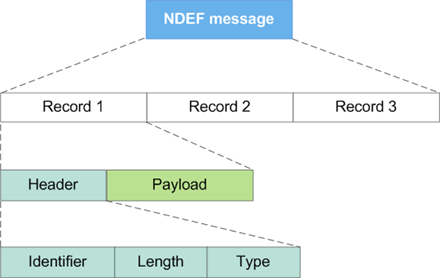
\includegraphics[width=0.5\textwidth]{NDEF_Format.png}
	\caption[Caption for LOF]%
		{NDEF Message Format\footnote{\url{http://www.developer.nokia.com/Community/Wiki/Understanding_NFC_Data_Exchange_Format_(NDEF)_messages}}}

\end{minipage} 
\end{figure}

Specifically, the Android system offers the ability to read and write NFC tags for passive mode, and beam NDEF messages from one device to another with Android Beam\footnote{\url{http://developer.android.com/guide/topics/connectivity/nfc/nfc.html}} for active mode. 

\subsection{Android Intents}
The core components of an Android application are activated through messages called intents.\footnote{\url{http://developer.android.com/guide/components/intents-filters.html}} Intents are used for inter-application and intra-application communication by sending messages with relevant information about operations to be performed to various applications.  

When NFC is enabled and the screen is unlocked, Android devices will always be searching for input from an NFC tag or device. When the device discovers an NFC tag, an intent is sent to the phone with information including which application is most appropriate to handle the data contained in the NFC tag. This information is processed by Android's special tag dispatch system to determine which activity to launch. In the case that more than one application can handle the type of data contained in the tag, the phone will open a prompt for the user to choose among the several applications; however, if there is only one application, the phone will automatically launch this application and process the tag. It turns out that through NFC one can force some phones to parse images, videos, contacts, office documents, call arbitrary phone numbers and even open up web pages in the browser, all without user interaction.  

\subsection{Android Permission System}
Android applications run in a sandbox which allows areas of the system to be isolated and thus limit access to the security-related parts of the Android API. However, access to these resources can be granted to an application if the developer requests the appropriate permissions in the application's manifest. Android developers are expected to use least-privilege with their permission requests: limit the permissions requested to only those that are absolutely necessary for the function of their applications. By analyzing the use of permissions, one can learn about the potential vulnerabilities introduced in an application. \TODO{Which we do later...}

\subsection{Threat Model}
As with any new technology, comes the potential for vulnerabilities within the system. Our paper attempts to analyze the potential threats that this new technology may introduce and how the coding practices of NFC applications relate to these threats. We focus predominantly on the ability of an attacker to force a device to scan a malicious tag. However, we consider other threat models including writing sensitive data to an insecure tag, eavesdropping on the data transferred over the NFC connection, and creating a malicious NFC application. 

\subsubsection{Malicious Tags}
It is possible to have a device scan a tag and perform the action specified by the tag without any user interaction, as mentioned previously. If an attacker can scan a tag unnoticed by the user, then the attacker can force the device to perform an arbitrary NFC action simply by writing it as part of a malicious tag. This opens the opportunity to have a phone open an arbitrary web url in the browser or call a specified phone number. 

If the url is malicious in any way, opening it in the browser can cause... \TODO{issues should be talked about here. Talk about how the malicious application might have access to the sensitive information on the phone itself or corrupt the phone in some way. I am not entirely sure what to say here.} 

If the attacker has the ability to automatically have the phone call a specified number, then a tolled number could easily be inserted and thus result in a monetary loss on the part of the user. This is a direct and obvious vulnerability in any application the calls an arbitrary phone number specified by a tag. An example of an application that does so is Samsung's Tectile application which, when scanning a tag with a phone number and directions to call this number, will do so without any further consideration. 

\subsubsection{Privacy Concerns}
Several NFC applications have the possibility of writing information to an NFC tag.
This means that users have the ability to write anything they want to their own tags.
It may be beneficial for some users to use these tag writing applications to write sensitive or critical information to tags they keep in specific locations.
However, if encryption is not used, an attacker who can gain access to these tags will have unfettered access to their information.
NFC is also used as a means of initiating connections on higher-bandwidth media (eg. bluetooth), but if this connection handover is interfered with then an attacker may be able to listen in on the new connection.

\TODO{An example of this might be... }. If the attacker was ever able to gain access to these tags, there is no security stopping him/her from reading the tag and viewing the sensitive content. 

\subsubsection{Eavesdropping}
In Securing Near Field Communication, Kortvedt, proves that it is possible to eavesdrop on NFC communication using simple equipment and methods. Since the NFC communication protocol does not offer any security or encryption itself, it is up to the developer to implement or use encryption to secure the data within the application's code. 

\TODO{I think the part below is irrelevant}
%\subsubsection{Malware}
%The last threat model we consider is that of an attacker creating his/her own malicious application. Given the fact that a majority of users ignore the permissions requested in a given application, an NFC application could easily request unnecessary and misleading permissions that give access to sensitive information from the phone itself. The application could then have access to such things as the contacts list, phone data, emails, and more. If the application also had some way to relay this information back to the attacker, for example, permission to access the Internet, then all of the user's information would be compromised. Since several NFC applications require multiple permissions, a user might not be as easily able to discern the necessary permissions or understand what the permission is being used for, thus making it more likely for the user to simply trust the application. However, this is possible for applications outside of NFC specific ones, and thus we choose not to focus on this attack. 
%
%\TODO{How is this different than any other application? Talk more about that. More NFC applications need certain permissions than normal applications, so a user giving access to certain resources might be more likely?}


\section{Related Work}
Close range radio wave communication has existed for some time, but the application of NFC in mobile phones is a recent development and still growing in popularity.
The NFC Forum\footnote{\url{http://www.nfc-forum.org/}}, which publishes NFC standards\footnote{\url{http://www.nfc-forum.org/specs/spec_list/}} and best practices, was only formed in 2004.
%NFC also relies on the interface and protocol specification\footnote{\url{http://www.iso.org/iso/catalogue_detail.htm?csnumber=38578}} published in 2004.
The relative youth of this field has resulted in many aspects remaining largely unexplored.
In this section we present relevant past work in the area of NFC security, as well as mobile phone application security in general.

\TODO{cite the signed ndef papers}

Kortvedt's ``Securing Near Field Communications''\cite{kortvedt2009} presents a view of NFC vulnerabilities and privacy concerns which remains largely unchanged since the paper's publication.
%Kortvedt explains a means of intercepting NFC data, even outside of the advertised 10 cm range. %, as well as existing attempts at providing a cryptographically secure interface for NFC communication.
%Some applications employ cryptography (the majority being payment applications), but mostly as a means of authenticating users and thwarting malicious users. %, but no current secure-NFC framework enjoys widespread use.
Kortvedt proposes a framework which attempts to provide solutions for establishing a secure channel with mutual authentication via NFC, but it has not gained widespread adoption.
He suggests using a centralized key authority for distributing keys, which we believe is impractical and unscalable, given that both tag authors and application authors may wish to distribute keys, and users should be able to choose which authors they trust.
%We also seek to analyze the issue of providing a simple, secure NFC API for casual and inexperienced application developers.
We, on the other hand, seek to provide a decentralized mechanism for trusting and granting trust to a user-defined set of NFC tag authors.

One major foray into the analysis of network-level NFC vulnerabilities was presented by Charlie Miller at BlackHat 2012\cite{miller2012}.
%Miller employs fuzz testing to evaluate the security of both the NFC protocol layer implemented on various mobile phones, and subsequently to evaluate network-level security.
%Miller discusses the successes of fuzzing in identifying various NFC messages which will crash a device.
%Further, Miller provides evidence that carefully crafted NFC payloads can do much more than just crash a device--in some cases phones can be forced to parse arbitrary data or open web pages without user interaction.
Miller employs fuzz testing to show that carefully crafted NFC payloads can do much more than just crash a device---in some cases phones can be forced to parse arbitrary data or open web pages without user interaction.
Miller's work provides a wide analysis of the NFC attack surface, but our research will seek to provide much more depth in the exploration of application-level vulnerabilities.

RFID, a precursor to and superset of NFC, has also raised several security issues in the past.
Though RFID is a much older technology, it is remains relevant as both the foundation for NFC, and as a technology which is still employed in various applications (most prominently touch-activated credit cards).
Heydt-Benjamin et al.\cite{heydtbenjamin2007} discuss issues involved in early generation deployments of RFID credit cards, and were successfully able to initiate various attacks on three major RFID enabled credit cards (including attacks which access private information or enable arbitrary purchases by the attacker).
Such attacks remain important considerations due to the growing prominence of smartphone payment applications  (such as Google Wallet), so we keep all of these vulnerabilities in mind as we explore NFC security vulnerabilities.
This paper presents some countermeasures, but some may be impractical (such as shielding) and others can be improved upon due to more flexible computing options of smartphones.
%
%"Security in NFC, Strengths and Weaknesses" (http://events.iaik.tugraz.at/RFIDSec06/Program/papers/002%20-%20Security%20in%20NFC.pdf) discusses general security issues with NFC (beyond the scope of just mobile phones). The paper discusses threats of eavesdropping, data corruption, data modification, data insertion, and man-in-the-middle attacks (though MITM is dismissed as practically impossible). The paper recommends establishing a secure channel between devices in order to prevent such attacks, and provides valuable discussion of how this channel would work. The paper does not, however, provide an implementation (as the purpose of the paper was to illustrate general NFC issues). As our focus is restricted to Android devices, we have the ability to recommend and implement Android-specific solutions.
%
%Francis et al. (http://eprint.iacr.org/2011/618.pdf) discuss the potential for relay attacks on NFC transactions, and implement a software version of this attack which can be used on an NFC-enabled device. A relay attack exploits the assumption that two devices engaged in an NFC transaction are actually adjacent (by placing a proxy in between the two devices). This is a serious potential exploit which must be defended against by any security-conscious application (as it may allow for arbitrary credit card purchases, for example). The paper suggests several potential counters to such attacks; our analysis examines how popular applications employ relay-attack countermeasures, and to what degree they are effective.
%
%"Using QR tags to Attack SmartPhones (Attaging)" presents a discussion of potential attacks which leverage scanning QR codes (Which can then open malicious links). The attacks made possible by malicious QR codes may in many cases be possible via NFC; some NFC applications will open arbitrary links transmitted, or load other content. An attacker could provide a malicious NFC tag which causes the user's phone to navigate to a malicious link (the user may not even be aware of this action, as was previously discussed). In addition to new potential exploits and leakage of private data resulting from NFC applications, previously encountered attacks may also be possible.
%
%Analysis of smartphone applications in general (though we restrict our focus to Android devices, as iPhones do not yet offer NFC) is a much more thoroughly explored field, and several projects provide valuable insight into application testing.
%
%TaintDroid (http://static.usenix.org/event/osdi10/tech/full_papers/Enck.pdf), in order to evaluate privacy leakage, surveyed the 50 most popular free applications on the Android marketplace. This approach provided valuable data regarding how private data is handled by common Android applications, and presents a good technique for large-scale application evaluation. Surveying popular NFC applications will be an important facet of our project, and the TaintDroid approach was able to gather highly representative data of the application area. We intended to leverage a similar approach in order to gather useful data regarding common NFC usage and potential leakage of information over NFC channels.
%
%There are several other tools for both static and dynamic analysis of Android applications, including Droidbox (http://code.google.com/p/droidbox/), which attempts to provide thorough analysis of an application, including its information leakage, data sent over the network, and use of Android cryptography operations, for example. Analysis such as this is valuable for determining whether or not an application even attempts to prevent information leakage when NFC transmission is used.
%
%While RFID technology and Android application analysis have both been explored, there has been very limited exploration of Android-specific NFC applications, and their potential vulnerabilities. We leverage this previous exploration to provide large-scale analysis of NFC applications, vulnerabilities, and coding practices, as well as to recommend best practices for preventing NFC attacks.

\todo{A bit on certificate authorities, perhaps?}

\url{http://www.nfc-forum.org/resources/white_papers/Using_ECQV_ECPVS_on_NFC_Tags.pdf}: elliptic curve signatures

\url{http://www.nfc-forum.org/apps/group_public/download.php/9052/doi_10.1109_NFC.2011.9.pdf}: security flaws in signature spec

\url{http://www.auto.tuwien.ac.at/bib/pdf_TR/TR0156.pdf}: bachelor's thesis, security overview

\todo{anything in analysis goes into background}
%\section{Analysis of Apps}
%* Intro: Why analyze
%** general coding practices re: NFC
%** what practices contribute to vulnerabilities of NFC apps
%** As for as we know, no broad analysis of NFC app level stuff
%** provide suggestion for NFC app devs (we are in a unique position in that this tech is up and coming)

%\subsection{Application Characteristics}
%*** tiny - have a specific function and only does one specific thing given a tag. These only require a small subset of permissions. 
%\\
%*** superapps - use a lot of permissions and perform several different actions ranging from reading and writing tags, to handling monetary transactions, performing actions on the phone, or transferring musics, pictures, or other data.
%
%\subsection{Static Analysis}
%* static
%\subsubsection{Permissions}
%* current apps, what permissions do they use - ML Classifier here
%\subsubsection{Taint Tracking}
%trace where data read from NFC tags is ended
%** other static tools? 
%\subsubsection{Crypto/Eavesdropping}
%\TODO{Eavesdropping - Talk about more in analysis portion when we discuss the use of crypto within application's code - the fact that developers aren't using known crypto libraries means they are either implementing crypto themselves or not securing their data at all} 
%** Overwriting tags- do apps in general 0 out prior data, or not?
%
%\subsection{Dynamic Analysis - might not exist}
%* dynamic
%** taintdroid
%** droidblaze
%
%\subsection{Manual Analysis}
%* manual
%** looked at source code of ~10 applications
%** played with apps
%** trace exec paths if possible
%** BEAM
%*** If you scan an app, it'll take you to the app store

\section{Proposed Solution}
% talking points:
% trust model
% authentication
% key management
% usability
% 
% * Goals/non-goals
% * architecture
% ** distributed authentication
% *** generalizable to arbitrary inputs to phone?
% 
% * Goals
% 
% As a user
% I want to be able to verify a tag came from a given author
% In order to ensure I am not acting on malicious inputs
% 
% As a user
% I want to be able to keep track of tag authors
% In order to expand the scope of tags I can trust
% 
% As a user
% I want to be able to verify my own tags
% In order to ensure use my own tags
% 
% As a user
% I want to be able to encrypt my own tags
% In order to ensure no one else can read my tags
% 
% As a user
% I want to keep the identities of trusted tag authors correct
% In case if good authors go bad
% 
% As a user
% I want to report malicious tag authors
% To warn other users of bad authors
% 
% As a tag author
% I want to share my key with a user
% To prevent others from impersonating me
% 
% ** integrity
% ** authentication

We propose a novel solution which provides way for users to only read tags that have been written by tag providers that they trust.
There are three types of actors in our security model: application authors, tag authors, and users.
The main threat model we consider is when malicious tag authors trick users into scanning malicious tags.
In order to prevent users from reading malicious tags, we force tags to prove their authenticity through the use of digital signatures.
Users or applications will then be able to act on tags based on whether or not they trust the tag author or whether the tag can successfully prove its authenticity.

Under our proposal, each NFC tag contains an additional record containing a tag author's signature.
Each tag author has a unique key pair comprising a public and a private key.
The tag author generates the signature record from his or her private key and the other data records on the tag.
The signature record can be validated with the tag author's public key, which is can be shared with users.

Users may add the public keys of any tag authors they trust, allowing tags written by those authors to be automatically used by applications which implement the protocol.
Keys are stored on the Android phone.
\TODO{Verify that this is right. Or figure out how the scheme works with sharing keys between apps?}
While we did not restrict access to the key file, we believe that it would be trivial to modify the Android kernel to restrict applications with special permissions to read or write the key file.

\subsection{Key Distribution and Management}
% How to get keys?
% * Go to website of tag author you trust, DL their key
% * see it for the first time (good info in prompt?)
% * No signature: different prompt
% 
% Prompts:
% * disable all pmopts
% * never allow this key?
% * allow key once
% * allow key always
% * allow all keys
% 
% * We should alway state why we make any choice

For usability reasons, we provide two ways for a user to add a trusted key: (1) a public key can be stored on the tag itself, or if storage space on the tag is limited, (2) a tag may contain a URL pointing to the location of a public key.
In both cases, a user only needs to scan a tag with his or her phone in order to receive a public key.
While the application author can determine how it wants to handle unrecognized or untrusted public keys, we recommend the following scheme for maximum usability and security:
If a user does not already have a tag's public key, they are prompted to either (1) accept the tag and store the public key, (2) accept the tag this time only and do not store the public key, or (3) reject the tag.

A user must trust the source of a public key, so we recommend that if a tag author chooses to distribute a key through a tag, that the tag is in a location that is constantly monitored so that malicious users cannot simply replace the tag.
Similarly, if a tag author chooses to distribute a key through a URL, we recommend that the author chooses an easily verifiable location for the key, such as on an SSL-protected, well-recognized domain.
As a special case, if a user wishes to write their own tags, we can automatically add the user's public key to the user's key file when initially generating a key pair.  
We believe that these methods of key distribution cover the majority of application use cases. \TODO{Why?}

To revoke a key, a user can simply remove the offending key from the key file.
To improve usability for the most common use case, we provide a method for revoking the most recently added key, as a user will usually know whether a tag is malicious moments after adding a new public key.

\subsection{Caveats}
% * Non goals
% ** confidentiality of tag data
% ** ignoring malicious applications
% ** no central authority
% ** not ensuring security of key exchange

We do not make any privacy guarantees with the scheme that we propose.
A tag author cannot assume that any private data written to a tag will only be read by authorized users, since the data on the tag in unencrypted.

Similarly, our scheme assumes that applications are not malicious.
If an application is malicious, then securing tag data will not protect users from malicious behavior since we rely on an application to correctly authorize tag data.

\section{Implementation}
We implemented our authentication system as an Android library that Android developers can include and access in their projects.
Our current implementation provides both means of writing and reading tags using our authentication scheme, allowing developers of both tag-reading and tag-writing applications to benefit from increased security.
We present this implementation as a proof-of-concept; ideally, such additions to the Android NFC stack would be implemented at OS-level.
There are several advantages to kernel modifications, which are discussed below.

\subsection{SignedNdef}
The Android NFC API provides access to \texttt{Ndef}, which allows access to the NDEF message contained on a tag.
Our API offers \texttt{SignedNdef}, which offers the same methods as \texttt{Ndef}, but implicitly handles authentication.
Android developers can use the API we developed for interfacing with a \texttt{SignedNdef} object, which we designed to closely mimic the existing official Android \texttt{Ndef}\footnote{http://developer.android.com/reference/android/nfc/tech/Ndef.html} object for reading and writing NDEF tags.
The approach we use for authentication is to use the Elliptic Curve Digital Signature Algorithm (ECDSA) to sign the contents of a message, thus allowing the reader of a tag to verify that the tag was written by a trusted tag author.
Our data format for secure NDEF tags appends an extra NDEF record to the end of an NDEF message.
This record contains both information regarding the public key used for signing (discussed in further detail below) and the ECDSA signature of the original Ndef message.
\TODO{Show figure for the new record format}

\subsection{Key Management}
Users need to be able to add and remove keys from their base of trusted authors (either manually, or through a tag reader application).
For our API, we use Android's \texttt{SharedPreferences}, which provides persistent key-value storage.
Our current implementation provides a unique instance of this key storage (a \texttt{KeyFile}) to an individual application (ie. a given application can only access and modify its own keys).
Key sharing between applications is a useful feature which would be simpler to implement securely at OS-level.
When a user reads a tag, the tag's signature record will either contain a public key in its entirety, or contain a URI pointer to a public key.
If this public key has been added to the Key File, it is considered trusted, otherwise, the user must add this key.
\TODO{``tag providers''? or ``tag authors''? what should we name them?}
When a user writes a tag using this API, the private key for the phone is accessed and a ECDSA signature is generated and appended.

\subsection{Application Flow}
On instantiation, a \texttt{SignedNdef} object will attempt to open up the list of authorized keys saved on the Android device.
It provides methods for opening, closing, reading, and writing NDEF-formatted tags by delegating to a private instance of the \texttt{Ndef} class.
In addition, it will automatically enforce the security protocols described earlier.
When reading a tag, it will query the \texttt{KeyManager} to find a public key which matches the signature of the signed Ndef tag.
If it can locate a valid public key which matches the signature, it will transparently return the non-signature records on the tag.
In case of any errors, failure to verify the signature or failure to locate a valid public key, reading the tag will throw an exception.
\TODO{include figure for application flow}

\subsection{Cryptographic protocols}
One issue regarding the storage of additional authentication data on an NFC tag is the limited size of the tag.
To address this, we use ECDSA, which is able to use smaller keys to provide the same security as DSA with a larger key.
For example, a 160-bit ECDSA key provides the same security level as a 1024-bit DSA key.
\TODO{verify the above, which is from wikipedia}
We use SHA-2 for the hashing function.
\TODO{currently we actually use DSA with SHA1, not ECDSA with SHA2}

\subsection{Recommendations for Kernel Implementation}
Implementing this scheme at OS-level will allow for simpler sharing of keys between applications, by providing a single, shared Key File.
We recommend an additional application permission in order to make a modification of this Key File; this will provide greater control over which applications have been granted permission to influence the set of trusted tag authors.
This implementation would also allow Android itself to display messages to the user, in order to centralize and standardize any necessary error reporting or warnings.


\section{Fine-grained Access/New Trust Model}
* idea: associate a tag type or permission with a key in order to trust authors with specific NFC abilities/actions (i.e. let Safeway open URLs, let Yelp call phone numbers)

* Why it's better than the other solution

* Contrary arguments to our solution

* Why it's still fast and usable for a developer and a user

* Central Authority - implicit trust vs. every user gets to specify what they want to trust
 
* ACLs for NFC tags - mapping of which application are allowed to read which data types from nfc tags signed by certain public keys (ACL: this thing can do this)

\section{Evaluation}
\subsection{Space Performance}
\subsection{Usability}
\subsection{Security}
* simplicity/overhead for user (warning message?)
* how many apps can benefit from this?
* applicability
** do 3 case studies (examples of applying it to an application)
** do it on github
* How many additional lines of code required for using API?

* (performance (time+space))
* security of this scheme
** bits of security (e.g. signature size)
** assumptions/foundations (e.g. secure key distribution)
** key storage on Android phones can't be tampered with

* LIMITATIONS

* key add/revoke
** app perm to add
** app perm to remove
** done via syscalls, i.e. android holds this
*** some intent?
** some way for app developer to add centralized repo of keys
** automatic get key

* Does phone already have a pub key pair?
* backwards compatibility
** Read NDEF standards and how Android handles them

brainstorm                         works for                           bad
- NDEF record/type for signature   updated os
                                   app viewing finite \# records
- length exclused signature        above                               violates standards
  + above                          app viewing variable \# of records   


\section{Discussion}
* this seems like it's throughout the paper already?

\section{Recommended User Study}
* user study, human testing
* overhead imposed by warnings/approvals
** delves into usable security

\section{Future Work}
* compression/optimization
* OS perms, kernel mods to support this
* application sharing and how to do this well

\section{Conclusion}

\section{Acknowledgements}

\section{References}

\bibliographystyle{abbrv}
\bibliography{cs261}

\end{document}
